\documentclass[12pt, a4paper]{article}
\usepackage[utf8]{inputenc}
\usepackage[spanish]{babel}
\usepackage{amsmath, amssymb}
\usepackage{graphicx}
\usepackage{hyperref}
\usepackage{geometry}
\geometry{margin=2.5cm}

\title{Proyecto 2: Opciones Call Ventana y Modelo Black-Scholes}
\author{}
\date{}

\begin{document}

\maketitle

\section{Simulación del Proceso de Valor}

En esta sección se describe la implementación computacional del modelo de Black-Scholes para la simulación del proceso de valor de un activo subyacente $S(t)$. El algoritmo genera trayectorias aleatorias utilizando un método de discretización temporal paso a paso.

\subsection{Metodología Matemática}

El modelo asume que el precio del activo sigue un Movimiento Browniano Geométrico (MBG), el cual se puede discretizar mediante la siguiente ecuación recursiva:
\begin{equation}
    S_{i+1} = S_i + \mu S_i \Delta t + \sigma S_i \sqrt{\Delta t} Z_i
\end{equation}
donde:
\begin{itemize}
    \item $S_i$ es el precio del activo en el instante $t_i$.
    \item $\mu$ es la tasa de tendencia (drift).
    \item $\sigma$ es la volatilidad del activo.
    \item $\Delta t$ es el tamaño del incremento de tiempo finito.
    \item $Z_i$ es una variable aleatoria que sigue una distribución normal estándar, es decir, $Z_i \sim \mathcal{N}(0,1)$. El término $\sqrt{\Delta t} Z_i$ modela el incremento en un proceso de Wiener estocástico ($\Delta W_i$).
\end{itemize}

El vector temporal avanza de manera determinista según la relación:
\begin{equation}
    t_{i+1} = t_i + \Delta t
\end{equation}

\subsection{Algoritmo Implementado}

El algoritmo fue codificado utilizando el lenguaje de programación Python. Se empleó la librería \texttt{numpy} para el manejo eficiente de arreglos numéricos y la generación de variables aleatorias, así como \texttt{matplotlib} para la visualización del proceso.

El procedimiento ejecutado computacionalmente se describe en los siguientes pasos:

\begin{enumerate}
    \item \textbf{Inicialización de Parámetros Escalares:} Se definen los valores clave para la simulación: el número de pasos temporales $N$, el incremento de tiempo $\Delta t$, el precio inicial del activo $S_0$ en el tiempo $t_0$, la tendencia $\mu$ y la volatilidad $\sigma$.
    
    \item \textbf{Preparación de Estructuras de Datos:} Se crean dos arreglos (vectores) de longitud $N+1$ pre-inicializados con ceros para almacenar de forma iterativa el tiempo $t$ y los precios $S$. Se asignan las condiciones de borde iniciales: $t_0$ en la primera posición del arreglo de tiempo y $S_0$ en la primera posición del arreglo de valor.
    
    \item \textbf{Ciclo Iterativo de Simulación:} Se ejecuta un bucle donde una variable $i$ toma los valores desde $0$ hasta $N-1$. Por cada iteración:
    \begin{itemize}
        \item Se actualiza el tiempo asignando a la posición $i+1$ el valor $t_i + \Delta t$.
        \item Se extrae un número aleatorio $Z_i$ proveniente de una distribución normal estándar mediante el generador estocástico.
        \item Se calcula y almacena el nuevo precio del activo $S_{i+1}$ incorporando el término determinista de tendencia ($\mu S_i \Delta t$) y el término estocástico de volatilidad ($\sigma S_i \sqrt{\Delta t} Z_i$).
    \end{itemize}
    
    \item \textbf{Evaluación de Múltiples Trayectorias:} Con el objetivo de comprender visualmente la dispersión y naturaleza aleatoria del proceso, la lógica del algoritmo se encapsula en una función que permite generar múltiples trayectorias independientes con los mismos parámetros base.
    
    \item \textbf{Visualización Gráfica:} Finalmente, se construyen gráficos comparativos en los que se grafican los vectores $(t, S)$ para diferentes cantidades de simulaciones (por ejemplo, 1, 3 y 10 caminos simultáneos). Esto permite evidenciar cómo, a pesar de compartir el mismo punto de partida y ecuación gobernante, cada trayectoria en el modelo de Black-Scholes es única debido a los choques estocásticos de la variable $Z_i$.
\end{enumerate}
\subsection{Resultados y Análisis}

A continuación se presentan las figuras generadas por la simulación computacional. Estas gráficas muestran diferentes trayectorias del proceso estocástico, evidenciando el efecto de la volatilidad y la tendencia a lo largo del tiempo.

\begin{figure}[htbp]
    \centering
    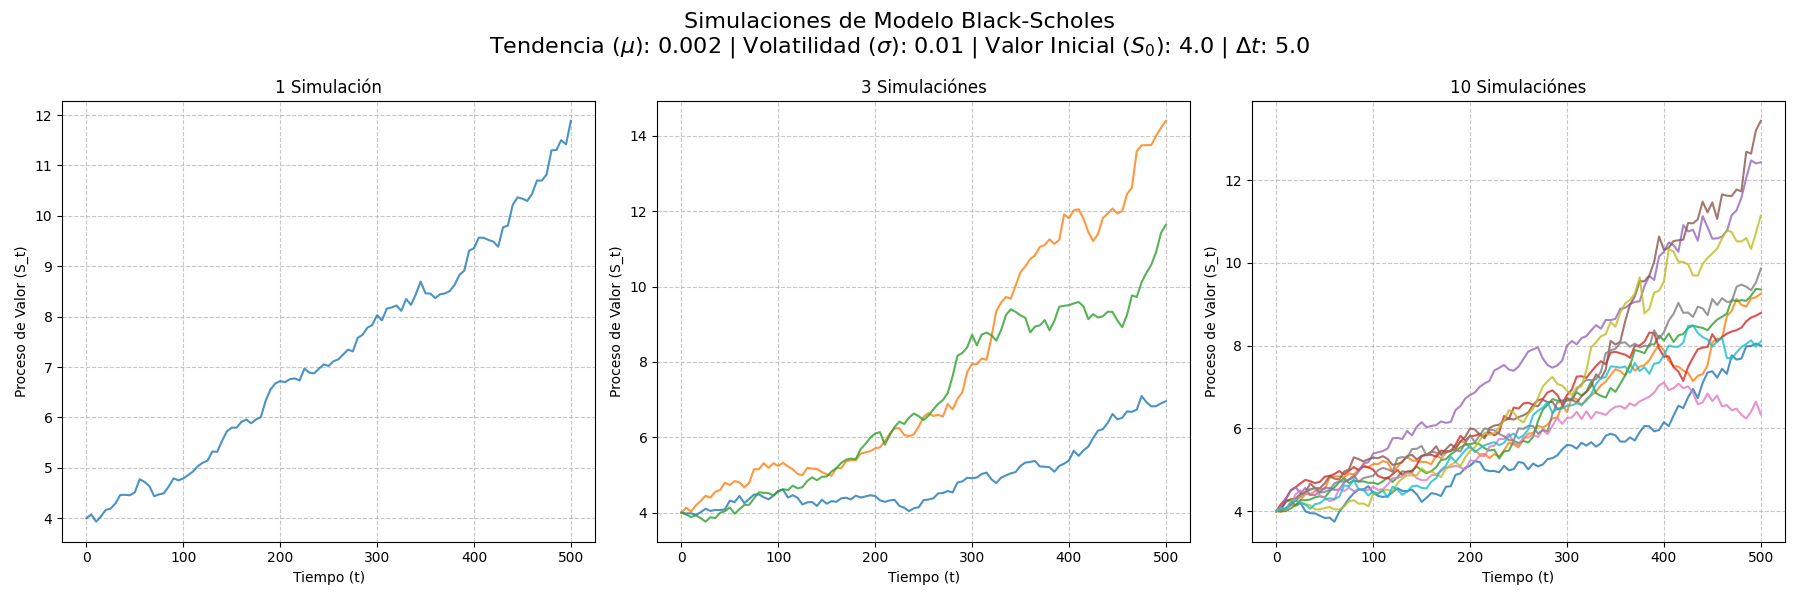
\includegraphics[width=\textwidth]{../Figuras/Punto1_Figura1.png}
    \caption{Simulación del proceso de valor.}
    \label{fig:punto1_1}
\end{figure}

\begin{figure}[htbp]
    \centering
    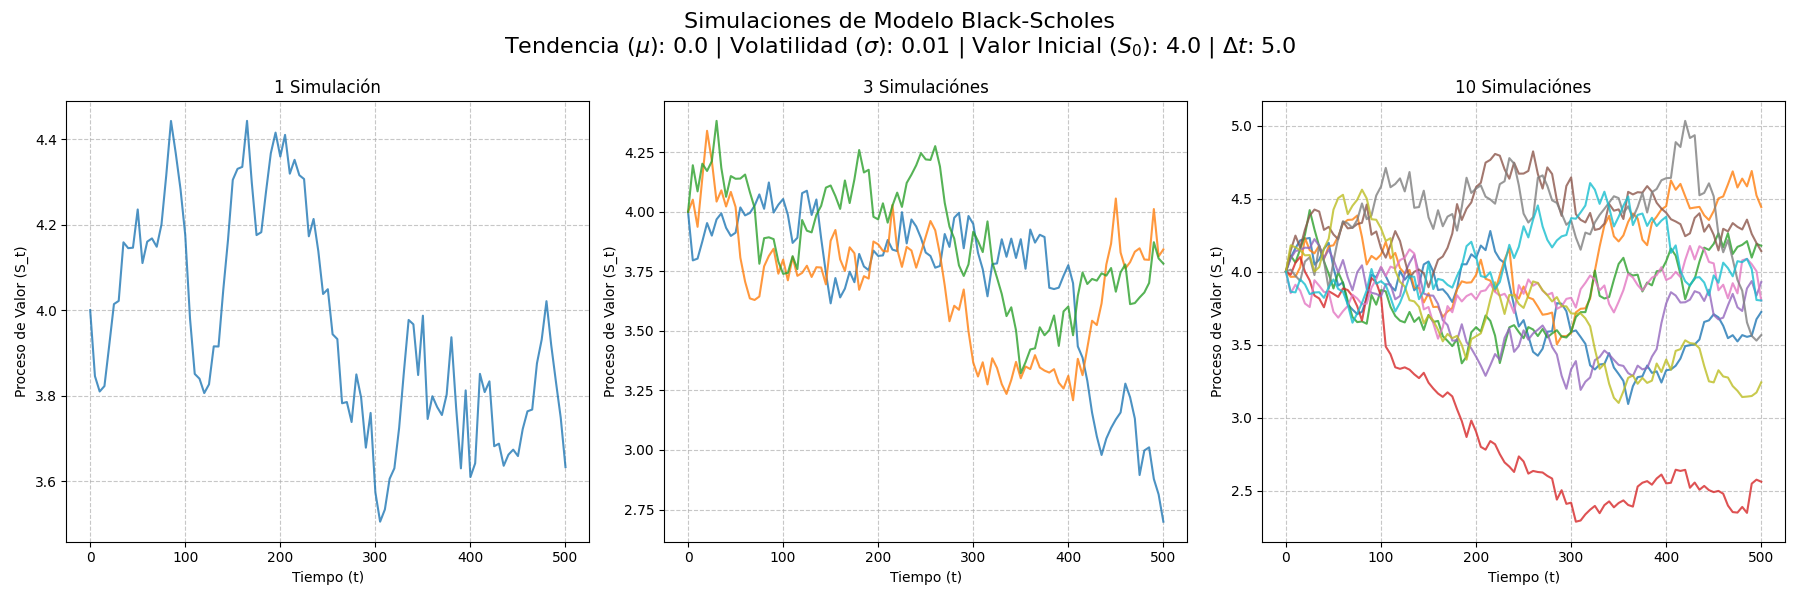
\includegraphics[width=\textwidth]{../Figuras/Punto1_Figura2.png}
    \caption{Simulación del proceso de valor.}
    \label{fig:punto1_2}
\end{figure}

La Figura 1 ilustra un escenario con tendencia positiva ($\mu = 0.002$), donde el activo exhibe un crecimiento sistemático a largo plazo impulsado por el drift, el cual logra imponerse sobre las fluctuaciones aleatorias generadas por la volatilidad. Por el contrario, la Figura 2 presenta una tendencia nula ($\mu = 0.0$), resultando en un proceso puramente estocástico donde los precios oscilan de manera simétrica alrededor del valor inicial de 4.0, dejando el destino del activo bajo el control exclusivo de la incertidumbre y el ruido del mercado. El contraste fundamental radica en que, mientras en la Figura 1 la tendencia actúa como una fuerza directriz que inclina la balanza hacia la rentabilidad esperada, en la Figura 2 la ausencia de este sesgo permite que la volatilidad disperse los resultados sin una dirección preferente, evidenciando cómo el parámetro de drift es el único responsable de transformar un camino aleatorio errático en una trayectoria con una progresión económica definida.

\section{Derivación Analítica de la Opción Call Ventana}

\subsection{Ecuaciones de Black-Scholes}

El modelo de Black-Scholes parte de la premisa axiomática de que el valor del activo subyacente, $S(t)$, evoluciona de acuerdo con una Ecuación Diferencial Estocástica (EDE). Esta ecuación involucra un parámetro de tendencia constante (drift) $\mu$ y una volatilidad $\sigma$ constante:

\[ dS = \mu Sdt + \sigma SdW \]

Donde $dW$ representa el diferencial de un Proceso de Wiener (o movimiento browniano estándar), el cual introduce la aleatoriedad en el mercado.

Buscamos una función $C = C(S, t)$ que determine el valor justo de la opción "Call Ventana" en el tiempo $t$ dado un precio del subyacente $S$. Dado que $S$ es una variable estocástica, no podemos usar el cálculo diferencial ordinario para encontrar el diferencial $dC$; debemos recurrir al cálculo estocástico mediante el Lema de Ito.

El Lema de Ito equivale a una expansión en series de Taylor de primer orden respecto al tiempo $t$ y de segundo orden respecto a la variable espacial $S$:

\[ dC \cong \frac{\partial C}{\partial t} dt + \frac{\partial C}{\partial S} dS + \frac{1}{2} \frac{\partial^2 C}{\partial S^2} (dS)^2 \]

Sustituyendo $dS$ y sabiendo por las reglas del cálculo estocástico que $(dS)^2 \cong \sigma^2 S^2 dt$ (dado que los términos de orden superior como $(dt)^2$ y $dt \cdot dW$ se desvanecen en el límite, y $(dW)^2 = dt$), obtenemos la dinámica del valor de la opción:

\[ dC = \left( \mu S \frac{\partial C}{\partial S} + \frac{1}{2} \sigma^2 S^2 \frac{\partial^2 C}{\partial S^2} + \frac{\partial C}{\partial t} \right) dt + \sigma S \frac{\partial C}{\partial S} dW \]

Esta ecuación nos dice cómo cambia el valor de la opción, pero aún depende del término aleatorio $dW$.

El objetivo central de Black y Scholes fue encontrar una regla matemática de valoración que estuviera libre de la incertidumbre del mercado. Para lograrlo, construimos un portafolio $\Pi$ que consiste en poseer una posición larga en la opción ($+C$) y una posición corta en una cantidad $\Delta$ del activo subyacente ($-\Delta S$):

\[ \Pi = C - \Delta S \]

Calculamos el cambio infinitesimal en el valor de este portafolio, asumiendo que $\Delta$ se mantiene constante durante el diferencial de tiempo $dt$:

\[ d\Pi = dC - \Delta dS \]

Sustituyendo nuestras expresiones previas para $dC$ y $dS$, y factorizando para agrupar por separado los términos deterministas ($dt$) y los términos estocásticos ($dW$), llegamos a:

\[ d\Pi = \left( \mu S \left( \frac{\partial C}{\partial S} - \Delta \right) + \frac{1}{2} \sigma^2 S^2 \frac{\partial^2 C}{\partial S^2} + \frac{\partial C}{\partial t} \right) dt + \left( \frac{\partial C}{\partial S} - \Delta \right) \sigma S dW \]

Para blindar completamente el portafolio contra el riesgo de mercado, debemos eliminar la fuente de aleatoriedad. Esto obliga matemáticamente a anular el coeficiente que multiplica al proceso de Wiener $dW$. Por lo tanto, elegimos estratégicamente:

\[ \Delta = \frac{\partial C}{\partial S} \]

Al imponer esta condición, el riesgo se elimina por completo y la dinámica del portafolio se simplifica a una ecuación puramente determinista:

\[ d\Pi = \left( \frac{1}{2} \sigma^2 S^2 \frac{\partial^2 C}{\partial S^2} + \frac{\partial C}{\partial t} \right) dt \]

Dado que el portafolio $\Pi$ ahora está matemáticamente libre de riesgo (su varianza es cero para el instante $dt$), los principios de no arbitraje dictan que debe rendir exactamente lo mismo que un activo libre de riesgo (como un bono gubernamental) que paga una tasa de interés continua $r$. Por ende, su crecimiento debe satisfacer:

\[ d\Pi = r\Pi dt \]

Sustituimos la definición original del portafolio $\Pi = C - \Delta S$ (recordando que $\Delta = \frac{\partial C}{\partial S}$) en esta nueva ecuación:

\[ d\Pi = r \left( C - S \frac{\partial C}{\partial S} \right) dt \]

En este punto, contamos con dos expresiones distintas para el cambio determinista del portafolio $d\Pi$. Al igualar ambas expresiones, obtenemos:

\[ \left( \frac{1}{2} \sigma^2 S^2 \frac{\partial^2 C}{\partial S^2} + \frac{\partial C}{\partial t} \right) dt = r \left( C - S \frac{\partial C}{\partial S} \right) dt \]

Cancelando el diferencial temporal $dt$ a ambos lados y trasladando todos los términos a un solo lado de la igualdad, llegamos a la formulación final de la Ecuación Diferencial Parcial de Black-Scholes:

\begin{equation}
    \frac{\partial C}{\partial t} + \frac{1}{2} \sigma^2 S^2 \frac{\partial^2 C}{\partial S^2} + r S \frac{\partial C}{\partial S} - r C = 0
\end{equation}

Como se ha demostrado, la derivación es completamente agnóstica a si la opción es estándar o tipo ``ventana''; la EDP modela estrictamente la física financiera de la réplica libre de riesgo del subyacente.

\subsection{Condiciones de Frontera}

La condición final establece el valor de la opción en el momento exacto en que expira el contrato. Es decir, determina la función de pago (payoff).

Para una opción Call europea estándar, el derecho de compra otorga un valor de $\max(S-E, 0)$. Sin embargo, la opción ``Ventana'' introduce una restricción categórica: el contrato solo se puede ejercer si el precio final $S(T)$ cae estrictamente dentro del intervalo $[E_1, E_2]$.

Por lo tanto, la función de pago se define como una función a trozos (o usando una función indicadora). Matemáticamente, la condición en $t=T$ es:

\[ C(S, T) = \begin{cases} \max(S - E, 0) & \text{si } E_1 \leq S \leq E_2 \\ 0 & \text{si } S < E_1 \text{ o } S > E_2 \end{cases} \]

Si asumimos lógicamente que el límite inferior de la ventana es al menos el precio strike ($E_1 \geq E$), el término $\max(S-E, 0)$ dentro de la ventana siempre será positivo, y la condición puede reescribirse simplemente como $S - E$ dentro del rango $[E_1, E_2]$.

Debemos evaluar qué ocurre con el valor de la opción si el precio del activo subyacente colapsa a cero antes del vencimiento.

Aquí entra en juego la distribución log-normal del precio $S(t)$. Una propiedad clave de este modelo estocástico es que el estado $S=0$ es un límite absorbente; si el precio cae a cero, la variación estocástica se anula (el término $\sigma S dW$ se vuelve cero) y el activo pierde todo su valor y no puede recuperarse.

Dado que el precio permanecerá en cero, es absolutamente imposible que el precio al vencimiento $S(T)$ alcance la barrera inferior de activación $E_1$ (asumiendo $E_1 > 0$). La probabilidad de que la variable log-normal transite de 0 a un valor dentro de la ventana es nula. En consecuencia, el derecho de compra carece por completo de valor. Matemáticamente, se expresa como:

\[ C(0, t) = 0 \]

Finalmente, debemos evaluar qué ocurre con el valor de la opción si el precio del activo subyacente se valoriza muy alto en un valor $S_{\infty}$ antes del vencimiento. Esta condición difiere drásticamente de una opción Call estándar y es donde la naturaleza de la ``Ventana'' y la distribución log-normal cobran mayor relevancia.

En un Call estándar, si $S \to \infty$, la opción inevitablemente se ejerce y la condición asintótica es $C(S,t) \to S - Ee^{-r(T-t)}$. Sin embargo, para la opción Ventana, el contrato se invalida si $S(T) > E_2$. Si evaluamos el límite cuando el precio actual del activo $S(t)$ crece hacia el infinito, el centro de la distribución log-normal (su media) se desplaza infinitamente hacia la derecha.

\begin{itemize}
    \item La varianza de la distribución log-normal en un tiempo finito $T-t$ es limitada.
    \item Como la varianza es finita, a medida que $S(t) \to \infty$, la probabilidad de que el precio colapse drásticamente para caer por debajo del umbral máximo $E_2$ antes del tiempo $T$ tiende estrictamente a cero.
\end{itemize}

Dado que la probabilidad de que la variable aleatoria aterrice dentro del intervalo de activación $[E_1, E_2]$ se desvanece, la opción pierde toda posibilidad de ser ejercida. Esto impone un comportamiento asintótico en forma de límite hacia cero:

\[ \lim_{S \to \infty} C(S, t) = 0 \]

\subsection{Solución Analítica mediante la Ecuación del Calor}

Partimos de la Ecuación Diferencial Parcial (EDP) de Black-Scholes deducida previamente. El primer objetivo es eliminar los coeficientes variables ($S$ y $S^2$) que acompañan a las derivadas espaciales e invertir el flujo del tiempo para transformarlo en un problema de valor inicial. Definimos las siguientes sustituciones:

\begin{enumerate}
    \item \textbf{Dimensión espacial:} Adimensionalizamos el precio del activo respecto al precio strike $E$ usando un logaritmo: $S = E e^x \implies x = \ln(S/E)$.
    \item \textbf{Dimensión temporal:} Invertimos el tiempo y lo escalamos con la varianza: $\tau = \frac{\sigma^2}{2}(T - t)$.
    \item \textbf{Valor de la opción:} Escalamos el valor de la opción: $C(S, t) = E v(x, \tau)$.
\end{enumerate}

Aplicando la regla de la cadena, relacionamos los diferenciales originales con las nuevas variables:

\begin{itemize}
    \item $\frac{\partial C}{\partial t} = -\frac{E \sigma^2}{2} \frac{\partial v}{\partial \tau}$
    \item $\frac{\partial C}{\partial S} = \frac{E}{S} \frac{\partial v}{\partial x}$
    \item $\frac{\partial^2 C}{\partial S^2} = \frac{E}{S^2} \left( \frac{\partial^2 v}{\partial x^2} - \frac{\partial v}{\partial x} \right)$
\end{itemize}

Sustituimos estos operadores en la EDP de Black-Scholes original:

\[ -\frac{E \sigma^2}{2} \frac{\partial v}{\partial \tau} + \frac{\sigma^2 S^2}{2} \left[ \frac{E}{S^2} \left( \frac{\partial^2 v}{\partial x^2} - \frac{\partial v}{\partial x} \right) \right] + r S \left[ \frac{E}{S} \frac{\partial v}{\partial x} \right] - r E v = 0 \]

Dividiendo toda la expresión entre el factor común $\frac{E \sigma^2}{2}$ y reordenando, obtenemos una ecuación con coeficientes constantes:

\[ \frac{\partial v}{\partial \tau} = \frac{\partial^2 v}{\partial x^2} + (k - 1) \frac{\partial v}{\partial x} - kv \]

Donde definimos la constante adimensional $k = \frac{r}{\sigma^2/2}$.

La ecuación anterior aún contiene términos de primera derivada y proporción directa que debemos suprimir. Introducimos nuestra función objetivo final $u(x, \tau)$ mediante un factor integrante exponencial:

\[ v(x, \tau) = e^{\alpha x + \beta \tau} u(x, \tau) \]

Calculamos las derivadas de $v$ en términos de $u$:

\begin{itemize}
    \item $v_\tau = e^{\alpha x + \beta \tau} (\beta u + u_\tau)$
    \item $v_x = e^{\alpha x + \beta \tau} (\alpha u + u_x)$
    \item $v_{xx} = e^{\alpha x + \beta \tau} (\alpha^2 u + 2\alpha u_x + u_{xx})$
\end{itemize}

Al sustituir esto en nuestra ecuación anterior y dividir por $e^{\alpha x + \beta \tau}$, llegamos a:

\[ \frac{\partial u}{\partial \tau} = \frac{\partial^2 u}{\partial x^2} + (2\alpha + (k - 1)) \frac{\partial u}{\partial x} + (\alpha^2 - \beta + (k - 1)\alpha - k)u \]

Para que esta expresión colapse rigurosamente en la ecuación de difusión pura ($\frac{\partial u}{\partial \tau} = \frac{\partial^2 u}{\partial x^2}$), los coeficientes de $u_x$ y $u$ deben ser cero. Esto nos obliga a definir los parámetros:

\begin{enumerate}
    \item $2\alpha + (k - 1) = 0 \implies \alpha = \frac{1 - k}{2}$
    \item $\alpha^2 - \beta + (k - 1)\alpha - k = 0 \implies \beta = -\frac{(1 + k)^2}{4}$
\end{enumerate}

Bajo estas condiciones, hemos transformado exitosamente la ecuación a la Ecuación del Calor:

\begin{equation}
    \frac{\partial u}{\partial \tau} = \frac{\partial^2 u}{\partial x^2}
\end{equation}

Para resolver la ecuación del calor, necesitamos la condición inicial $u(x, 0) = g(x)$. Traducimos la condición de pago al vencimiento ($t=T \implies \tau=0$) de nuestra opción Ventana.

Sabemos que la opción solo se ejerce si $S \in [E_1, E_2]$ y su pago es $\max(S-E, 0)$. Matemáticamente, el pago será positivo solo si $S \ge E$. Por ende, la opción tiene valor en el dominio efectivo $S \in [\max(E_1, E), E_2]$. Para facilitar la notación, definamos el límite inferior efectivo como $S_{min} = \max(E_1, E)$.

\begin{itemize}
    \item Límite inferior en $x$: $x_1 = \ln(S_{min}/E)$
    \item Límite superior en $x$: $x_2 = \ln(E_2/E)$
\end{itemize}

La condición es $C(S,T) = E v(x, 0) = E e^{\alpha x} u(x, 0)$. Igualando al pago y despejando $u(x,0)$, obtenemos nuestra función $g(x)$:

\[ g(x) = e^{-\alpha x}(e^x - 1) = e^{(1-\alpha)x} - e^{-\alpha x} \quad \text{para } x \in [x_1, x_2] \]

La teoría de probabilidad y la física matemática nos dicen que la solución a este problema de valor inicial se encuentra mediante el valor esperado con respecto al núcleo del calor (una distribución normal):

\[ u(x, \tau) = \frac{1}{\sqrt{4\pi\tau}} \int_{-\infty}^{\infty} g(s) e^{-\frac{(x-s)^2}{4\tau}} ds \]

Sustituyendo nuestra $g(s)$ particionada, la integral se delimita y se divide en dos:

\[ u(x, \tau) = \underbrace{\int_{x_1}^{x_2} \frac{e^{(1-\alpha)s} e^{-\frac{(x-s)^2}{4\tau}}}{\sqrt{4\pi\tau}} ds}_{I_1} - \underbrace{\int_{x_1}^{x_2} \frac{e^{-\alpha s} e^{-\frac{(x-s)^2}{4\tau}}}{\sqrt{4\pi\tau}} ds}_{I_2} \]

Ambas integrales tienen la forma general $J(A) = \int_{x_1}^{x_2} \frac{1}{\sqrt{4\pi\tau}} e^{As - \frac{(x-s)^2}{4\tau}} ds$. Completamos el trinomio cuadrado perfecto en el exponente:

\[ As - \frac{(x-s)^2}{4\tau} = -\frac{1}{4\tau} (s - (x + 2\tau A))^2 + Ax + A^2\tau \]

Esto nos permite extraer los términos constantes y realizar el cambio de variable $w = \frac{s - (x + 2\tau A)}{\sqrt{2\tau}}$:

\[ J(A) = e^{Ax + A^2\tau} \frac{1}{\sqrt{2\pi}} \int_{w_1}^{w_2} e^{-\frac{w^2}{2}} dw = e^{Ax + A^2\tau} \left[ F_Z(w_2) - F_Z(w_1) \right] \]

Donde $F_Z$ es la Función de Distribución Acumulada de la normal estándar y los límites son $w_i = \frac{x_i - x - 2\tau A}{\sqrt{2\tau}}$.

Aplicamos este resultado general a $I_1$ (donde $A = 1-\alpha$) y a $I_2$ (donde $A = -\alpha$). Reconstruimos el precio de la opción $C(S,t) = E e^{\alpha x + \beta \tau} [I_1 - I_2]$.

Para el primer término ($I_1$), el coeficiente externo será $E e^{\alpha x + \beta \tau} e^{(1-\alpha)x + (1-\alpha)^2\tau} = E e^{x + (\beta + (1-\alpha)^2)\tau}$. Usando las definiciones de $\alpha$ y $\beta$, sabemos que $\beta + (1-\alpha)^2 = 0$. Por tanto, el coeficiente se reduce a $E e^x = S$.

Para el segundo término ($I_2$), el coeficiente externo será $E e^{\alpha x + \beta \tau} e^{-\alpha x + \alpha^2\tau} = E e^{(\beta + \alpha^2)\tau}$. Sabemos que $\beta + \alpha^2 = -k$. Sustituyendo $k$ y $\tau$, el coeficiente es $E e^{-r(T-t)}$.

Evaluación de los argumentos de $F_Z$: Al sustituir $x = \ln(S/E)$, $\tau = \frac{\sigma^2}{2}(T-t)$, $x_1 = \ln(S_{min}/E)$ y $x_2 = \ln(E_2/E)$, los argumentos $w_i$ toman la forma exacta de los parámetros $d_1$ y $d_2$ de Black-Scholes, pero evaluados en los límites de la ventana.

Para $I_1$ ($A = 1-\alpha$):
\[ w^{(1)}_i = \frac{\ln(S_i/S) - (r + \frac{\sigma^2}{2})(T-t)}{\sigma\sqrt{T-t}} = -d_1(S, S_i) \]

Para $I_2$ ($A = -\alpha$):
\[ w^{(2)}_i = \frac{\ln(S_i/S) - (r - \frac{\sigma^2}{2})(T-t)}{\sigma\sqrt{T-t}} = -d_2(S, S_i) \]

Donde $S_i$ toma los valores $S_{min}$ (para $w_1$) y $E_2$ (para $w_2$). Recordando la simetría de la normal estándar $F_Z(w_2) - F_Z(w_1) = F_Z(-w_1) - F_Z(-w_2)$, llegamos a la fórmula cerrada final:

\begin{equation}
    C(S,t) = S \left[ F_Z(d_1(S, S_{min})) - F_Z(d_1(S, E_2)) \right] - E e^{-r(T-t)} \left[ F_Z(d_2(S, S_{min})) - F_Z(d_2(S, E_2)) \right]
\end{equation}

Donde:
\begin{itemize}
    \item $S_{min} = \max(E_1, E)$
    \item $d_1(S, X) = \frac{\ln(S/X) + (r + \sigma^2/2)(T-t)}{\sigma\sqrt{T-t}}$
    \item $d_2(S, X) = \frac{\ln(S/X) + (r - \sigma^2/2)(T-t)}{\sigma\sqrt{T-t}}$
\end{itemize}

\subsection{Implementación Computacional de las Superficies}

La fórmula analítica deducida anteriormente fue implementada en el lenguaje de programación Python. El objetivo de este código es evaluar el precio justo de la opción en un rango continuo de precios del subyacente y tiempos al vencimiento para construir las superficies de valor del contrato.

La implementación consta de las siguientes características principales:
\begin{enumerate}
    \item \textbf{Cálculo de la Función de Valor:} Se programó la función \texttt{call\_ventana} que recibe como parámetros el precio actual $S$, el tiempo $t$, la tasa libre de riesgo $r$ (que asume el papel de la tendencia $\mu$), la volatilidad $\sigma$, y los límites espaciales del contrato $E$, $E_1$ y $E_2$.
    \item \textbf{Manejo de Condiciones Límite:} El código incorpora condicionales matemáticos estrictos que retornan un valor nulo ($C=0$) si el activo cae a cero, si las barreras hacen imposible el ejercicio ($S_{min} \ge E_2$), o si el tiempo evaluado es exactamente al vencimiento ($t \to T$), en cuyo caso simplemente aplica la función de pago (\textit{payoff}).
    \item \textbf{Vectorización Computacional:} Se utilizó el módulo \texttt{scipy.stats.norm} para calcular eficientemente la distribución normal acumulada $F_Z$. Posteriormente, la función fue vectorizada con \texttt{numpy.vectorize} para permitir la evaluación simultánea sobre una matriz de datos sin necesidad de bucles iterativos.
    \item \textbf{Generación de la Malla Tridimensional:} Se generó un dominio de evaluación bidimensional (\textit{meshgrid}) para el precio del subyacente $S \in [60, 140]$ y el tiempo $t \in [0, 1]$. La ecuación matemática deducida se evaluó sobre cada nodo de esta malla.
\end{enumerate}

Para evaluar el impacto de la tendencia en la valoración, se evaluaron los dos escenarios de simulación requeridos:
\begin{itemize}
    \item \textbf{Caso 1:} Tasa (tendencia) $r = 0.002$ y volatilidad $\sigma = 0.01$.
    \item \textbf{Caso 2:} Tasa (tendencia) $r = 0.0$ y volatilidad $\sigma = 0.01$.
\end{itemize}

A continuación, se presenta la gráfica resultante que ilustra la topología del valor del contrato $C(S,t)$ bajo ambas configuraciones, evidenciando cómo la variación sutil en la tasa libre de riesgo afecta la superficie de valoración en el tiempo.

\begin{figure}[htbp]
    \centering
    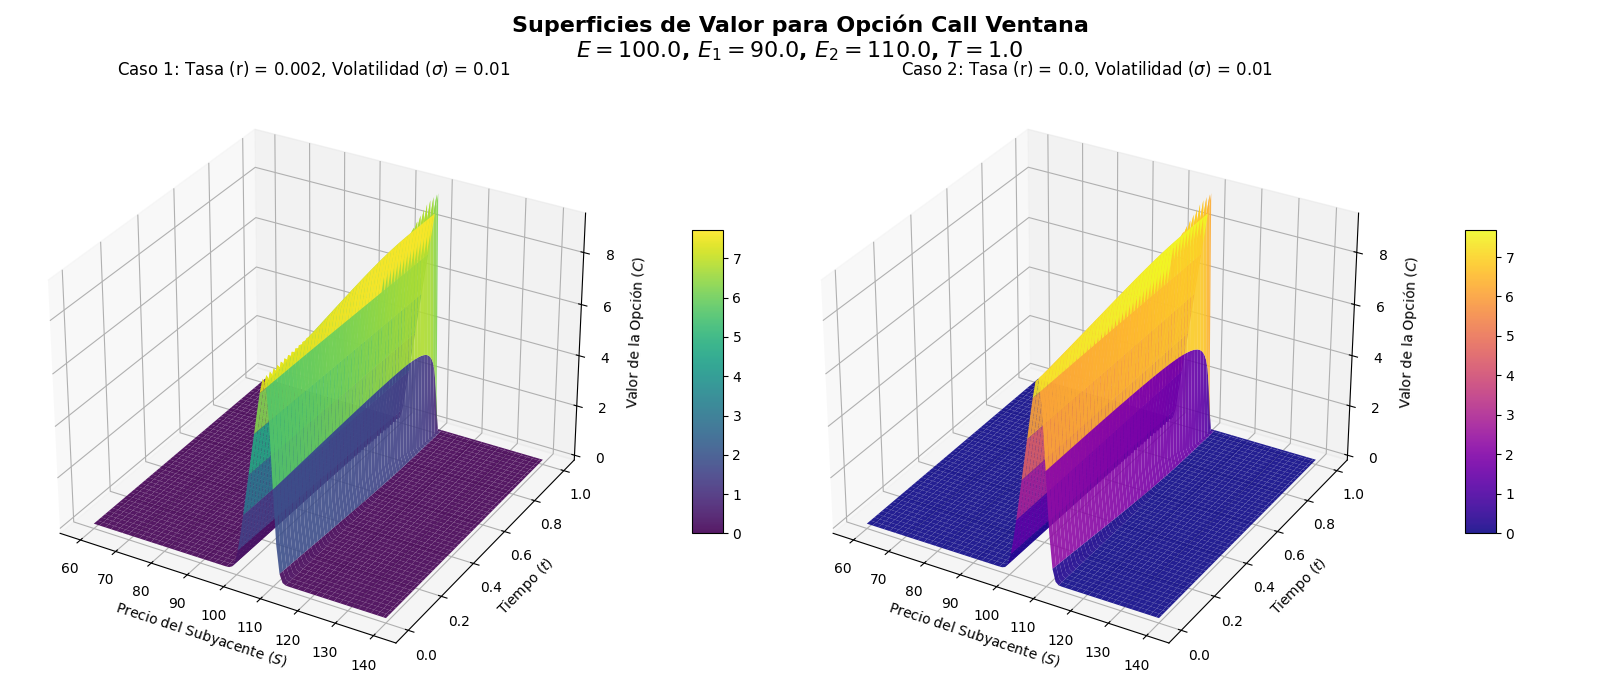
\includegraphics[width=\textwidth]{../Figuras/Punto2_Figura1.png}
    \caption{Superficies de Valor para la Opción Call Ventana. A la izquierda, la superficie bajo una tasa positiva $r=0.002$. A la derecha, la superficie cuando la tasa se anula $r=0.0$. La volatilidad es de $\sigma=0.01$ en ambos casos.}
    \label{fig:punto2_1}
\end{figure}

La figura 3 presenta las superficies de valoración para una opción Call Ventana bajo dos escenarios de tasas de interés, destacando la influencia crítica de los límites $E_1=90.0$ y $E_2=110.0$ sobre el valor del contrato. Se observa con rigor que el valor de la opción es nulo fuera del intervalo de activación, lo que valida las condiciones de frontera asintóticas donde la probabilidad de que el activo (que sigue una distribución log-normal) termine dentro de la ventana se desvanece en los extremos espaciales. La evolución temporal muestra cómo el perfil de la superficie se agudiza hacia el vencimiento ($T=1.0$), momento en el cual el valor converge a la función de pago $\max(S-E, 0)$ restringida al rango pactado, mientras que en tiempos anteriores la difusión térmica suaviza la "ventana", permitiendo que la opción tenga valor preventivo debido a la incertidumbre estocástica. El contraste entre el Caso 1 ($r=0.002$) y el Caso 2 ($r=0.0$) evidencia que incluso una tasa libre de riesgo mínima altera el plano de valoración al modificar el componente de descuento del portafolio replicante según el modelo de Black-Scholes.

\section{Construcción del Portafolio de Cobertura (Replicante)}

El tercer punto del proyecto requiere la integración de la simulación estocástica del activo subyacente (Punto 1) con la fórmula de valoración analítica de la opción ventana (Punto 2) para componer un portafolio de cobertura auto-financiado. La dinámica de este portafolio busca replicar exactamente la trayectoria del valor del contrato de la opción.

\subsection{Estructura del Portafolio}

De acuerdo con el modelo de Black-Scholes, la posición en un derivado puede ser perfectamente replicada construyendo un portafolio $\Pi_t$ que consista en:
\begin{enumerate}
    \item \textbf{Inversión en el Activo Subyacente $S$:} Mantener en cada instante de tiempo una cantidad de acciones equivalente a $\Delta_t = \frac{\partial C}{\partial S}$. Esto representa la sensibilidad direccional del precio de la opción ante fluctuaciones del subyacente.
    \item \textbf{Inversión en Activos sin Riesgo (Cuenta Bancaria):} Un capital $B_t$ depositado o prestado a la tasa de interés libre de riesgo $r$. Esta cuenta actúa como amortiguador de liquidez para financiar la compra o venta continua de acciones requeridas para el rebalanceo.
\end{enumerate}

Por lo tanto, el valor del portafolio replicante en cualquier instante de tiempo es:
\begin{equation}
    \Pi_t = \Delta_t S_t + B_t
\end{equation}

El objetivo de la cobertura dinámica es asegurar que $\Pi_t = C_t$ a lo largo de toda la trayectoria temporal del activo.

\subsection{Algoritmo de Simulación del Portafolio}

La implementación computacional de esta estrategia se llevó a cabo siguiendo esta metodología algorítmica paso a paso:

\begin{enumerate}
    \item \textbf{Simulación del Subyacente:} Se generó una trayectoria completa del precio del activo $S_t$ utilizando el esquema de Euler-Maruyama implementado en la Sección 1, configurado para simular $N = 252$ pasos a lo largo de $T = 1.0$ años con tendencia $\mu = 0.05$ y volatilidad $\sigma = 0.20$.

    \item \textbf{Inicialización del Portafolio ($t = 0$):} Se calcularon simultáneamente el valor teórico de la opción $C_0$ y la cobertura inicial $\Delta_0$ usando la fórmula analítica deducida. La posición en la cuenta bancaria se inicializó de modo que el portafolio valga exactamente el costo de la opción:
    \begin{equation}
        B_0 = C_0 - \Delta_0 S_0, \qquad \Pi_0 = \Delta_0 S_0 + B_0 = C_0
    \end{equation}

    \item \textbf{Evolución y Rebalanceo Dinámico:} Para cada paso de tiempo $t_{i} \to t_{i+1}$:
    \begin{enumerate}
        \item El capital en el banco devenga intereses continuos: $B_{\text{prev}} = B_{t_i} e^{r \Delta t}$.
        \item Se actualiza el valor del portafolio con el nuevo precio del activo: $\Pi_{t_{i+1}} = \Delta_{t_i} S_{t_{i+1}} + B_{\text{prev}}$.
        \item Se recalculan $C_{t_{i+1}}$ y $\Delta_{t_{i+1}}$ usando la fórmula de valoración analítica evaluada en el nuevo estado del mercado $(S_{t_{i+1}}, t_{i+1})$.
        \item Se rebalancea la posición en acciones. El diferencial de liquidez queda absorbido automáticamente por la cuenta bancaria:
        \begin{equation}
            B_{t_{i+1}} = \Pi_{t_{i+1}} - \Delta_{t_{i+1}} S_{t_{i+1}}
        \end{equation}
    \end{enumerate}

    \item \textbf{Estrategia de Aseguramiento (Covered Window Call):} Para demostrar la utilidad de la opción ventana como instrumento de cobertura, se construyó una segunda estrategia evaluada sobre $N_{\text{sim}} = 25$ trayectorias independientes con $\sigma = 0.05$ y ventana ampliada $[E_1, E_2] = [80, 120]$. En esta estrategia, el inversor:
    \begin{enumerate}
        \item Mantiene en su poder el activo subyacente (posición larga en $S_t$).
        \item Vende una opción Call Ventana al inicio del contrato, recibiendo la prima $C_0$ como ingreso inmediato.
        \item Deposita la prima en el banco, donde crece a la tasa $r$: $B_t = C_0 e^{r t}$.
    \end{enumerate}
    El valor del portafolio asegurado en cada instante es entonces:
    \begin{equation}
        \Pi_t^{\text{seg}} = S_t - C_t + B_t
    \end{equation}
    Al vencimiento, si el activo termina dentro de la ventana, la obligación de la opción vendida cancela la ganancia por encima de $E$, acotando el resultado final al valor fijo $E + B_T$. Si el activo termina fuera de la ventana, la opción expira sin valor y el inversor retiene tanto el activo como la prima con intereses, obteniendo un resultado superior.
\end{enumerate}

\subsection{Resultados y Análisis de Seguridad}

La figura~\ref{fig:punto3_1} presenta en un panel comparativo los resultados de las $N_{\text{sim}} = 25$ trayectorias simuladas bajo ambas estrategias. Los parámetros del escenario de aseguramiento son: tasa libre de riesgo $r = 0.05$, volatilidad $\sigma = 0.05$, precio strike $E = 100$ y ventana de activación $[E_1, E_2] = [80, 120]$.

\begin{figure}[htbp]
    \centering
    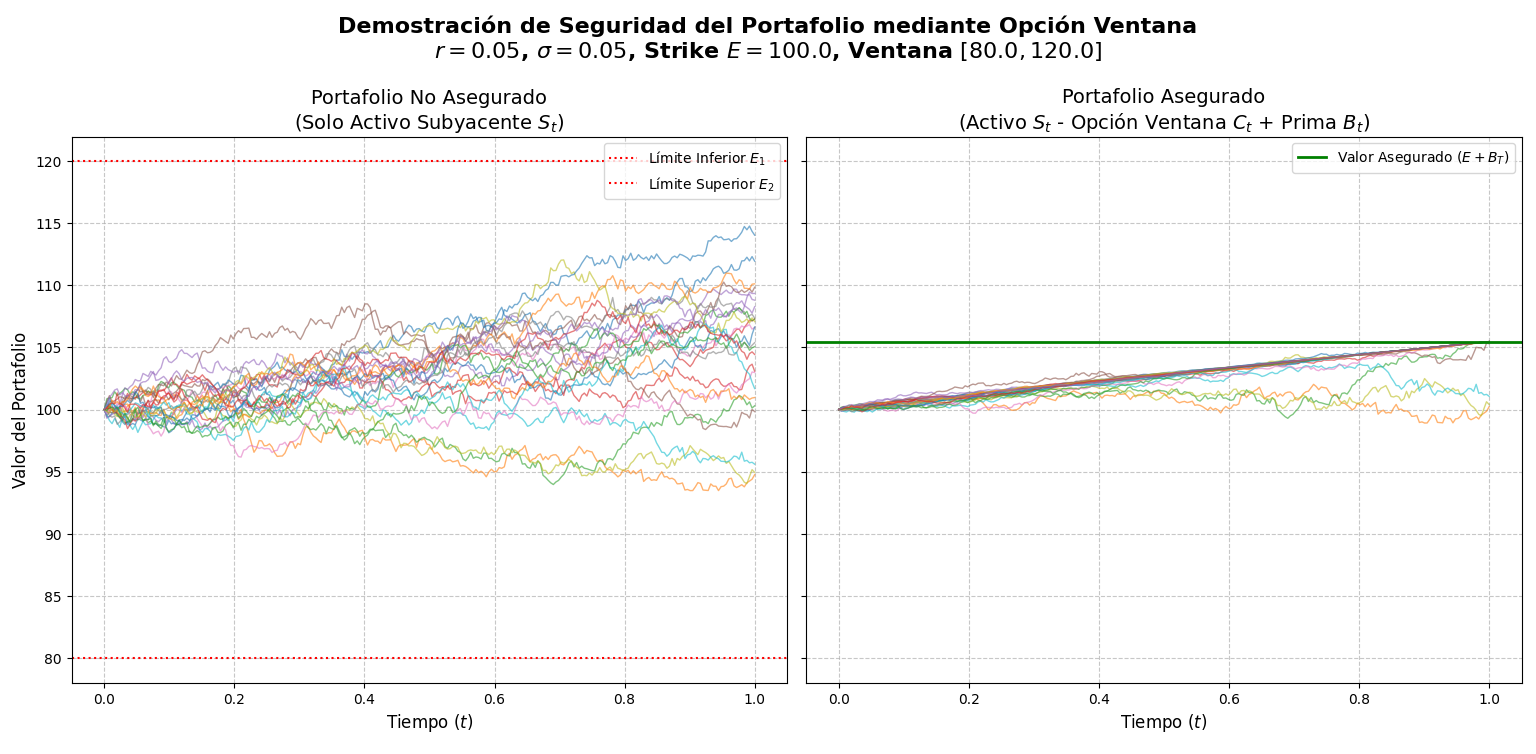
\includegraphics[width=\textwidth]{../Figuras/Punto3_Figura1.png}
    \caption{Comparación entre el portafolio no asegurado (izquierda) y el portafolio asegurado mediante una Covered Window Call (derecha) sobre 25 trayectorias simuladas.}
    \label{fig:punto3_1}
\end{figure}

\textbf{Panel izquierdo – Portafolio no asegurado:} Las trayectorias del activo subyacente $S_t$ exhiben una dispersión característica del Movimiento Browniano Geométrico. Las líneas punteadas en rojo marcan los límites $E_1 = 80$ y $E_2 = 120$ de la ventana de activación, evidenciando que el valor del portafolio puede oscilar libremente por encima o por debajo de dichos umbrales. El inversor queda completamente expuesto a la incertidumbre del mercado; una caída pronunciada del activo se traduce directamente en una pérdida equivalente del portafolio.

\textbf{Panel derecho – Portafolio asegurado (Covered Window Call):} Las mismas trayectorias, ahora ajustadas por la obligación de la opción vendida y la acumulación de la prima en el banco ($\Pi_t^{\text{seg}} = S_t - C_t + B_t$), convergen notoriamente hacia la línea verde horizontal que representa el valor asegurado $E + B_T$. La drástica reducción en la dispersión de los caminos es la demostración empírica de la utilidad de la opción ventana:

\begin{itemize}
    \item \textbf{Cuando $S_T \in [E_1, E_2]$:} La ganancia del activo por encima del strike $E$ queda exactamente capturada por la opción. El portafolio converge al valor fijo $E + B_T$, eliminando la varianza del resultado final.
    \item \textbf{Cuando $S_T \notin [E_1, E_2]$:} La opción expira sin valor ($C_T = 0$). El inversor conserva integralmente el activo $S_T$ más la prima $B_T$, obteniendo un resultado generalmente superior al del portafolio sin cobertura en estos escenarios extremos.
\end{itemize}

En consecuencia, la opción ventana reduce significativamente la varianza del valor final del portafolio, actuando como un mecanismo de estabilización que hace la estrategia de inversión más segura y predecible en cualquier escenario de mercado.

\end{document}
